\chapter{Práctica 1: Detección y seguimiento de caras con Sony Evi d100p}\label{cap.followface}
En este punto ya se han presentado contexto, los objetivos y las herramientas empleadas para llevar a cabo este proyecto, de manera que este capítulo está reservado para detallar el proceso de realización de la primera de las dos prácticas creadas en y para el entorno JdeRobot. Se explicará la infraestructura que le da soporte, el hardware involucrado y su forma de comunicación e interacción, el componente académico y la solución de referencia.

\section{Enunciado} \label{sec.enunciado}
Ésta práctica persigue que una cámara real sea capaz de seguir caras de personas. La cámara, evidentemente, sólo proporcionará sus imágenes captadas, a través de una capturadora de vídeo que irá proporcionando al nodo académico los frames  sucesivos. Además, la cámara dispondrá de dos actuadores de movimiento que controlarán su movimiento horizontal y vertical, a los cuales a partir de ahora llamaremos \textit{Pan} y \textit{Tilt} respectivamente.

Con todo ello, el alumno deberá programar un algoritmo de segmentación de caras de personas en la imagen y de control gradual en base a los datos que proporciona la imagen segmentada. Para ello, hay disponibles distintos elementos de \textit{debugging} o corrección de errores en el interfaz gráfico (GUI), ya que incluye espacios para la visualización de la imagen captada por la cámara y de la imagen segmentada, accesibles con dos sencillos objetos Python.

El algoritmo responde a un control reactivo, que en cada instante actuará en función de los datos de los sensores y sus propias variables internas. El control reactivo permitirá establecer en todo momento el movimiento del robot y responder ante situaciones imprevistas.

\section{Infraestructura}
En este apartado se introducirán los distintos componentes sobre los que se apoya la práctica, principalmente del hardware empleado y sus drivers controladores, pero también el componente académico, la interfaz y el código auxiliar.

\subsection{Cámara Sony Evi d100p}
El robot utilizado en esta práctica será la cámara Sony Evi modelo d100p, como el que se muestra en la Figura inferior (\textbf{Figura 4.1}), de la multinacional japonesa especializada en electrónica, \textit{gaming} y entretenimiento.

Este modelo cuenta con las siguientes características:
\begin{multicols}{2}
\begin{figure}[H]
  \begin{center}
    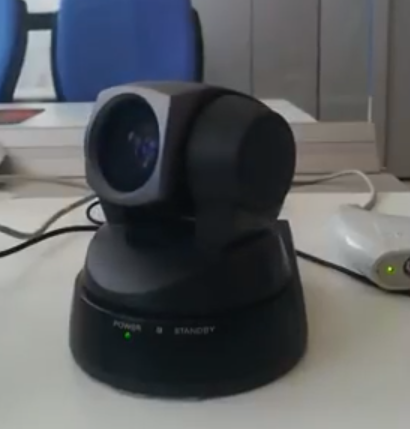
\includegraphics[width=0.88\linewidth, height=6.0cm]{figures/sonyevi.png}
		\caption{Cámara Sony Evi d1oop}
		\label{fig.sonyevi}
		\end{center}
\end{figure}
\begin{itemize}
	\item[--] 440,000 pixeles que permiten tomas en alta resolución.
	\item[--] Además de la acción de Pan y Tilt de alta velocidad, la mejora del mecanismo de reducción de ruido para vídeo en color. 
	\item[--] Posibilidad de operación desde computador a través de VISCA.
	\item[--] Buffer de mensajes que permite memorizar hasta 6 combinaciones de la posición y el estado de la cámara. 
	\item[--] Control remoto multifunción. 
	\item[--] Compatibilidad de comandos con modelos anteriores.
\end{itemize}
\end{multicols}

\begin{multicols}{2}
Dado que el hardware captura vídeo analógico, en combinación con la cámara se ha usado una capturadora de vídeo, que es un periférico de entrada cuya función es recibir señales de audio/video procedentes de dispositivos analógicos y convertirlas en señales digitales que puedan ser almacenadas o manipuladas por medio de software.
\begin{figure}[H]
  \begin{center}
    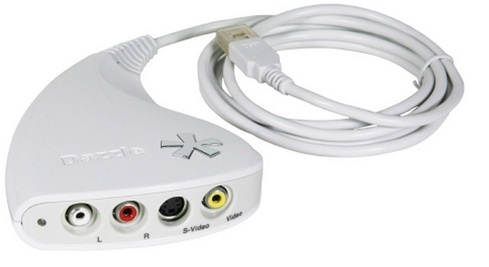
\includegraphics[width=0.55\linewidth, height=4.0cm]{figures/capturadora.jpg}
		\caption{Digitalizador Dazzle DVD Recorder}
		\label{fig.digitalizadora}
		\end{center}
\end{figure}
\end{multicols}
La capturadora utilizada es Dazzle DVD Recorder HD de la marca Pinnacle (\textbf{Figura 4.2}), y con conexión USB 2.0 con el ordenador. En cuanto a las capacidades del hardware en conjunto, nos interesan:

El valor de \textit{Pan} puede estar entre -164º y 164º y su velocidad puede tomar valores en un rango donde 1 es el mínimo y 24 es el máximo.

De forma análoga, el valor de \textit{Tilt} puede oscilar entre -30º y  30º, con velocidades en una escala de 1 a 20.

Por lo demás, la cámara utilizará \textit{drivers} para el acceso a la imagen y a los actuadores y para la comunicación con el nodo académico.

\subsection{Driver ROS usb\_cam}
El \textit{driver} usb\_cam interactúa con cámaras USB estándar (por ejemplo, SonyEvi d100p o Logitech Quickcam) utilizando libusb\_cam\footnote{\url{https://github.com/libusb/libusb/wiki}}, una biblioteca multiplataforma para acceso genérico a dispositivos USB, y publica imágenes bajo el formato de mensajes \textit{sensor\_msgs::Image}\footnote{\url{http://docs.ros.org/api/sensor\_msgs/html/msg/Image.html}} 
 de ROS. Además, utiliza la biblioteca \textit{image\_transport}\footnote{\url{http://wiki.ros.org/image\_transport}} para permitir el transporte de imágenes comprimidas.

A través de él obtendremos las imágenes que proporciona la cámara. Dado que es un driver de ROS, emplea la herramienta \textit{roslaunch}\footnote{\url{http://wiki.ros.org/roslaunch}}, que permite lanzar fácilmente múltiples nodos ROS de manera local o remota. Para ello, necesita un fichero de configuración XML como el siguiente: 

\begin{figure}[H]
  \begin{center}
    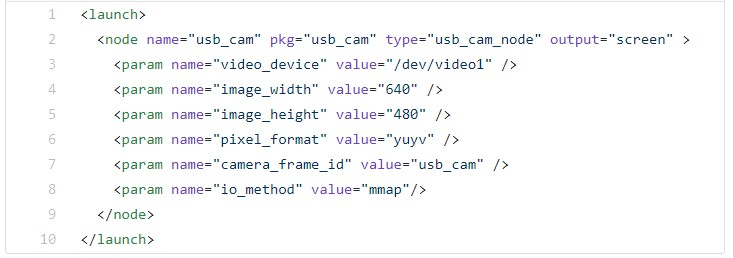
\includegraphics[width=0.99\linewidth]{figures/usbcamconf.jpg}
		\caption{Fichero de configuración de usb\_cam}
		\label{fig.usbcamconf}
		\end{center}
\end{figure}

En él deben especificarse los parámetros del nodo o nodos a establecer, así como los dispositivos sobre los cuales se lanza el nodo, en nuestro caso, la cámara (\textit{/dev/video1}).

\subsection{Driver Teleoperador Evicam}
El \textit{driver} Evicam ha sido desarrollado e incluido en la plataforma JdeRobot para poder teleoperar cámaras vía software a través de una conexión USB. En concreto, utiliza una interfaz ICE para poder controlarla a través de comandos de movimiento. 
El código fuente puede encontrarse en: 

\url{https://github.com/JdeRobot/JdeRobot/tree/master/src/drivers/evicam_driver}

Este driver debe lanzarse también con un fichero de configuración que indique el par \textit{IP:puerto} en el que la cámara espera órdenes y el dispositivo. Un ejemplo se muestra en la \textbf{Figura 4.4}:

\begin{figure}[H]
  \begin{center}
    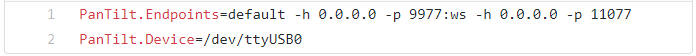
\includegraphics[width=0.99\linewidth]{figures/evicamconf.png}
		\caption{Fichero de configuración de evicam\_driver}
		\label{fig.evicamconf}
		\end{center}
\end{figure}

\section{Componente Académico}
El componente académico de esta práctica resuelve varias funcionalidades auxiliares que sirven de gran ayuda para poder abordarla:

\begin{enumerate}[label=\alph*)]
	\item Ofrece una interfaz gráfica al usuario que le ayuda a depurar su código; 
	\item Ofrece acceso a la cámara y a sus actuadores en forma de métodos simples (oculta el \textit{middleware} de comunicaciones con el hardware);  
	\item Incluye código auxiliar que no es el foco del algoritmo y que ayuda a programar la solución.
\end{enumerate}

El componente deja todo preparado para que el estudiante sólo tenga que incluir su código retocando el método \textit{execute} en el fichero \textit{MyAlgorithm.py}, e ir realizando las pruebas pertinentes.

El componente ofrece un API de cámara y actuadores al programador con el cuál acceder a la funcionalidad que necesita:

\begin{itemize}
	\item \textit{self.camera.getImage()}: devuelve la imagen capturada por la cámara activa (local o cámara usb).
	\item \textit{self.camera.setColorImage(img)}: método que recibe una imagen y la muestra en el espacio dedicado del interfaz para imágenes capturadas.
	\item \textit{self.camera.setThresholdImage(img)}: método que recibe una imagen tratada y la muestra en el espacio reservado en el GUI para imágenes filtradas, umbral o en blanco y negro.
	\item \textit{self.motors.getLimits()}: método a través del cual se pueden obtener los límites de Pan y Tilt (en grados).
	\item \textit{self.motors.setPTMotorsData(pan, tilt, panSpeed, tiltSpeed)}: método para enviar comandos de \textit{Pan} y \textit{Tilt} a la cámara. Necesita los valores respectivos en grados y la velocidad horizontal y vertical para alcanzar la posición fijada.
\end{itemize}

El nodo académico requiere un fichero de configuración que indique los \textit{endpoints} que utilizan la cámara y los motores PT. Este archivo tiene extensión \textit{.yml}, lo cual implica que debe seguir el formato de serialización de datos YAML, el cual produce datos fáciles de leer por humanos y máquinas para todos los lenguajes de programación. Tiene el siguiente aspecto:

\begin{figure}[H]
  \begin{center}
    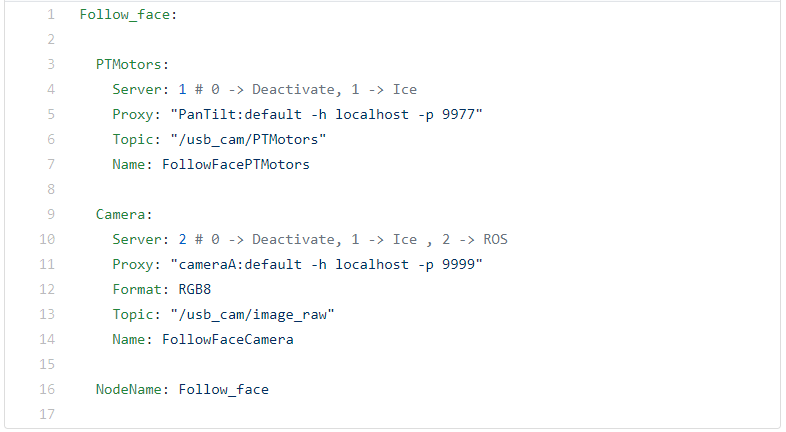
\includegraphics[width=0.99\linewidth]{figures/ymlfollowface.png}
		\caption{Fichero de configuración YAML de FollowFace}
		\label{fig.followfaceconf}
		\end{center}
\end{figure}

Se puede ver claramente que las interfaces empleadas por cámara y motores son distintas, siendo en el primer caso ROS y en el segundo ICE, como ya se explicó. Se observa también que puede incluir información adicional, como el formato de imagen.

En cuanto a la capacidad de cómputo para realizar todas las tareas simultáneamente, el componente emplea dos hilos de ejecución para agilizar la respuesta de los distintos módulos:
\begin{itemize}
	\renewcommand{\labelitemi}{$\to$}
	\item Hilo de algoritmo: se encarga del refresco de la ejecución del algoritmo, ya que este se ejecuta de modo cíclico. El tiempo de refresco de este hilo es muy importante, dado que su velocidad permitirá reaccionar ante situaciones imprevistas, y adaptar el movimiento de la cámara a la velocidad de movimiento de las personas, para poder seguir su cara. Es por eso que el tiempo de refresco es de 80 ms.
	\item Hilo de la interfaz gráfica de usuario (GUI): Este hilo es el encargado de actualizar la interfaz gráfica. También consta de los manejadores de eventos del GUI. El intervalo de actualización de la interfaz debe ser pequeño, ya que se tiene que mostrar las imágenes captadas por la cámara en forma de elemento vídeo, así como las imágenes segmentados en tiempo real. Por ello, se ha fijado el tiempo de refresco a 50 ms.
	
	Por último, el nodo académico incluye dos ficheros de descripción XML, que servirán de entrenamiento para los clasificadores que necesitaremos en la segmentación, explicados con mayor detalle en el apartado \textbf{4.4}. 
\end{itemize}

\subsection{Interfaz gráfica}
La interfaz gráfica de usuario (GUI) de la práctica sirve para representar información importante para desarrollar correctamente el algoritmo que lleve a la solución, además de para proporcionar funcionalidad básica para iniciar o para el algoritmo o para teleoperar la cámara. Se ha programado en Python con PyQt5, y es la mostrada en la \textbf{Figura 4.6}.

\begin{figure}[H]
  \begin{center}
    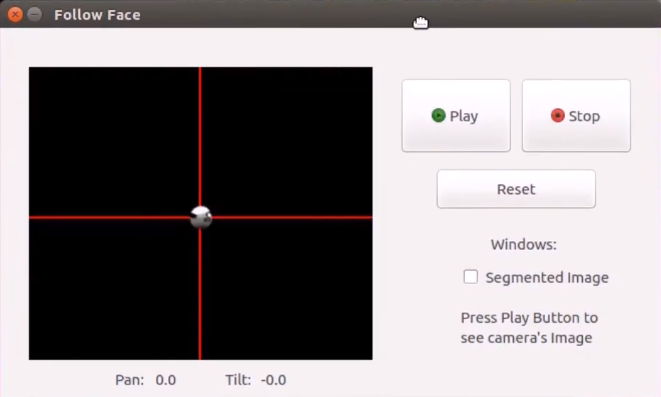
\includegraphics[width=0.99\linewidth]{figures/guifollowface.png}
		\caption{Interfaz Gráfica de Follow Face}
		\label{fig.guifollowface}
		\end{center}
\end{figure}

Se puede ver en ella, a la izquierda, el teleoperador para comprobar que el movimiento de la cámara este operativo. Se trata de un dial bidimensional que controla las componentes \textit{Pan} y \textit{Tilt} del robot. Únicamente será necesario mover el \textit{joystick} central en sentido vertical, para controlar el ángulo de \textit{Pan} y en sentido horizontal para fijar el \textit{Tilt}. Cuánto más se acerque el \textit{joystick} a los límites del teleoperador, más acentuado será el valor de la componente hacia la que se esté movimiento el mismo, ya sea éste un valor negativo si se mueve hacia abajo o hacia la izquierda, y positivo en caso de que se mueva hacia arriba o a la derecha. A su derecha, se han colocado varios botones cuya funcionalidad es la de iniciar el algoritmo, pararlo o resetearlo. Recordemos que la cámara dispone de un \textit{buffer} de mensajes, de manera que pulsar el botón Stop se traducirá en pausar el algoritmo, pero la cámara puede continuar en movimiento si había encolado mensajes, hasta que vacíe dicho \textit{buffer}. Inmediatamente debajo tenemos un \textit{check} que muestra la herramienta de imagen (\textbf{Figura 4.7}), en la cual se pueden ver las imágenes que provee la cámara (a la izquierda) y la imagen segmentada (a la derecha, en caso de haberla establecido):

\begin{figure}[H]
  \begin{center}
    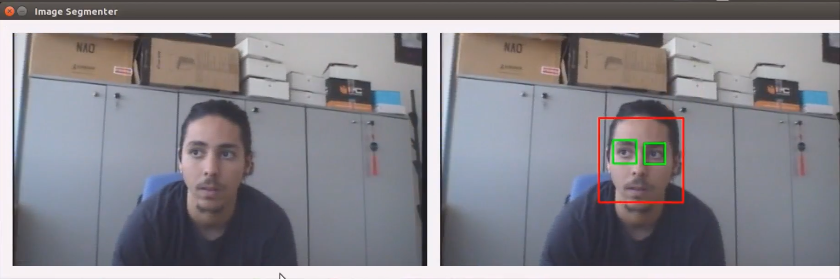
\includegraphics[width=0.99\linewidth]{figures/imagetool.png}
		\caption{Herramienta de imagen}
		\label{fig.imagetool}
		\end{center}
\end{figure}

\subsection{Código auxiliar: Clase CameraSegment}
Dentro del componente académico existe la clase \textit{CameraSegment}. Esta clase se ha creado por controlar y establecer la visualización de las imágenes que tienen que ver con la práctica, sustituyéndolas por imágenes negras si son nulas o estableciendo el vídeo capturado por la cámara y el vídeo segmentado creado y seleccionado por el programador.

El objeto \textit{self.camera} del cual dispone el algoritmo se construye a partir de ésta clase, por lo cual incluye algunos métodos propios además que los esperados por la cámara. Hablamos de las funciones que permiten mostrar las imágenes en el interfaz, descritas en \textbf{4.3}. Por tanto, actúa de nexo entre la herramienta de segmentación (\textit{segment widget}) y el algoritmo, proporcionando un API fácil de utilizar.

Por último, esta clase actúa de intermediario entre la cámara y el interfaz, conectando ambos componentes. Esto es necesario dado que las imágenes capturadas por la cámara y las que espera el interfaz no son completamente compatibles: para poder ser visualizadas, las imágenes deben redimensionarse para encajar en la aplicación gráfica.

\section{Solución de referencia}
Dado que el objetivo de la práctica es conseguir que el robot siga caras, la solución ha de contener un algoritmo de segmentación de imagen y otro de pilotaje, ambos respondiendo a un control reactivo. 
En esta sección, abordaremos brevemente los fundamentos de segmentación y detección de caras y el control gradual de hardware. Con ello construiremos una solución que se establecerá como solución de referencia en la plataforma, pero que sólo es uno de los muchos posibles métodos con el cual alcanzar el fin. El código quedara recogido en el fichero \textit{MyAlgorithm.py} que, como ya sabemos, es de naturaleza iterativa, de manera que en cada iteración se percibe, se actúa en consecuencia y se controla. Se habrá de escribir el método \textit{execute}, el cual debe contener la lógica que se ejecuta de manera cíclica en el \textit{thread} de algoritmo y computación.

\subsection{Fundamentos de la Detección de caras}
Las cámaras que incorporan los robots son una de las principales fuentes de información con las que cuentan, pero toda esta información es inútil sin la lógica que sea capaz de extraer la información relevante de la imagen. Incluso, algoritmos incapaces de diferenciar lo necesario de lo inane sólo conseguirán sobrecargar a la máquina de información inoperante, reduciendo su rendimiento e incluso llegando a producir comportamientos indeseados. Es por eso que es fundamental un buen algoritmo de detección de caras en la imagen, sobre todo cuando se trata de controlar un robot real con los datos extraídos y procesados. 

La detección de rostros se puede considerar como un caso específico de detección de “clases de objetos”. En la detección de clase de objeto, la tarea es encontrar las ubicaciones y tamaños de todos los objetos en una imagen que pertenecen a una clase determinada. Algunos ejemplos muy comunes en casos reales son torsos superiores, peatones y automóviles. De la misma forma, debemos ser capaces de encontrar caras en una imagen digital, sea cual sea su tamaño o ubicación en ella. Existen muchos algoritmos de detección de rostros para ubicar a una persona en una escena, algunos más fáciles y otros más complejos:

Cuando la imagen consta de un fondo monocolor simple o un fondo estático predefinido (conocido), es muy fácil detectar caras, dado que eliminar dicho fondo siempre tendrá como resultado los límites de la cara. Sin embargo, sabemos que en nuestro caso el robot debe comportarse correctamente en cualquier escenario, de manera que no es una solución válida.

Otra manera pasa por utilizar el color de piel típico para encontrar segmentos faciales, si se dispone de imágenes en color. La desventaja en este caso es que no funcionará con todo tipo de colores de piel, y que su robustez es mínima ante condiciones de iluminación variables. 

Existen otras técnicas basadas en la suposición de que las caras siempre estarán en movimiento en una secuencia de vídeo, de manera que calcular el área de movimiento se puede proporcionar una estimación. Todas ellas son poco robustas, pero juntas (y añadiendo algunos otros extras) se puede componer una buena aproximación a la solución. 

Sin embargo, y aunque resulte sorprendente, la forma de abordar esta tarea con mayor éxito es utilizar imágenes en escala de grises, con lo cual reducimos el coste computacional (requisito fundamental en aplicaciones en tiempo real). A su vez, hay varios métodos que las emplean, como son la detección basada en modelo, en emparejamiento de bordes por orientación, usando la distancia de Hausdorff\footnote{\url{https://en.wikipedia.org/wiki/Hausdorff_distance}},etc. Pero el más utilizado es mediante el uso de "clasificadores en cascada" encapsulado dentro de las técnicas de aprendizaje máquina que, utilizando características simples de Haar, puede producir resultados impresionantes.

El aprendizaje máquina o \textit{machine learning}, es una técnica empleada en el campo de las ciencias de computación y de estadística que aporta a las máquinas la capacidad de aprender en base a la observación de sucesos y decidir a partir de ellos. Así, un clasificador actúa de tal manera que “memoriza” la categoría asignada a un conjunto de sucesos conocidos (\textit{training group}), y a parir de ellos es capaz de realizar una inferencia o razonamiento inductivo, extrayendo características de los ejemplos del conjunto de entrenamiento y comparándolas con características de la misma naturaleza de nuevos ejemplos que entren al sistema. Únicamente habrá que dotar a la máquina de principios bien definidos que eviten que extraiga conclusiones inútiles. Con todo ello, una tarea extremadamente difícil de programar como podría ser reconocer todas y cada una de las caras existentes, se hace posible a través de este mecanismo capaz de clasificarlas sin haberlas visto antes.

Hay muchas motivaciones para usar características en la comparación en lugar de hacerlo con los píxeles directamente. La razón más común es que las características pueden codificar conocimiento del dominio ad-hoc, lo cual es difícil usando una cantidad finita de datos de entrenamiento. Para este sistema también hay una segunda motivación crítica para emplear características: el sistema basado en características funciona mucho más rápido que un sistema basado en píxeles. Estas características son las que se muestran en la siguiente imagen (\textbf{Figura 4.8}):

\begin{figure}[H]
  \begin{center}
    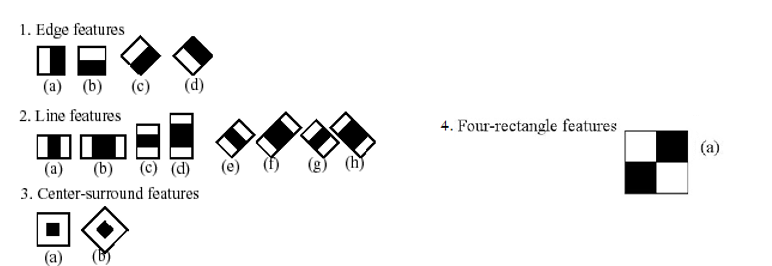
\includegraphics[width=0.99\linewidth]{figures/features.png}
		\caption{Características de comparación}
		\label{fig.features}
		\end{center}
\end{figure}

Cada “ventana” de las de la imagen se coloca en la imagen a segmentar para calcular una sola característica. Esta característica es un valor único que se obtiene al restar la suma de píxeles debajo de la parte blanca de la ventana de la suma de los píxeles debajo de la parte negra de la ventana. Así, todos los tamaños posibles de cada ventana se colocan en todas las ubicaciones posibles de cada imagen para calcular muchas características. 

\begin{figure}[H]
  \begin{center}
    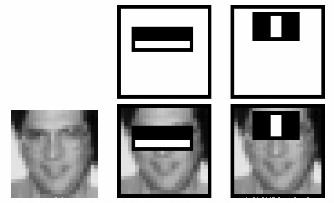
\includegraphics[width=0.69\linewidth]{figures/extraction.jpg}
		\caption{Extracción de características}
		\label{fig.extraction}
		\end{center}
\end{figure}

Por ejemplo, en la \textbf{Figura 4.9}, estamos extrayendo dos características. La primera se centra en la propiedad de que la región de los ojos a menudo es más oscura que el área de la nariz y las mejillas. La segunda característica se basa en la propiedad de que los ojos son más oscuros que el puente de la nariz.

Pero entre todas estas características calculadas, la mayoría de ellas son irrelevantes. Por ejemplo, cuando se usa en la mejilla, las ventanas se vuelven irrelevantes porque ninguna de estas áreas es más oscura o más clara que otras regiones en las mejillas, todos los sectores en ella son iguales. Por lo tanto, se debe descartar de inmediato las características irrelevantes y conservar únicamente aquellas importantes con una técnica llamada \textit{Adaboost} que selecciona solo aquellas características conocidas para mejorar la precisión de clasificación (cara / no cara) del clasificador. Finalmente, el algoritmo considera el hecho de que, en general, la mayor parte de la región en una imagen es una región sin cara. Teniendo en cuenta esto, es mejor idea tener un método simple para verificar si una ventana es una región sin rostro, y si no lo es, desecharla de inmediato y no volverla a procesar. Así el clasificador es capaz de enfocarse principalmente en el área donde exista una cara. Es por eso por lo que reciben el nombre de clasificadores en cascada (\textbf{Figura 4.10}), dado que se usan en primera instancia clasificadores simples para descartar esas áreas y luego clasificadores más complejos para eliminar falsos positivos.

\begin{figure}[H]
  \begin{center}
    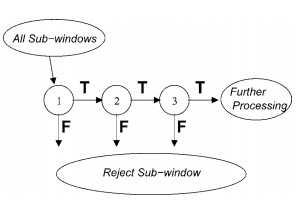
\includegraphics[width=0.50\linewidth, height=4cm]{figures/cascade.jpg}
		\caption{Clasificadores en cascada}
		\label{fig.cascade}
		\end{center}
\end{figure}

Esto permite reducir en gran medida la computación. Con ello, los sucesivos clasificadores son entrenados con las muestras que pasan las etapas anteriores. Un clasificador en cascada bien entrenado (incluyendo positivos y negativos), será capaz de identificar en una imagen dada si existen caras en ella, sea cual sea su origen, color, tamaño y posición con la parametrización adecuada.

\subsubsection{Clasificadores Máquina}
Como ya se ha visto, la manera escogida para abordar la tarea de detección pasa por utilizar un clasificador en cascada. 
Estudiando la librería OpenCV para Python, hemos encontrado la manera de crear entrenadores y detectores, los cuales se pueden entrenar de la forma que se desee. Además la librería incluye sistemas pre-entrenados para detectar facciones concretas de la cara como ojos, sonrisa, cejas e incluso la cara en sí.

Estos sistemas de entrenamiento se encuentran en ficheros XML provistos por la librería, dos de los cuales se han incluido en el nodo académico de esta práctica para poder abordarla siguiendo este método propuesto por  Paul Viola y Michael Jones en su \textit{paper}, \textit{"Rapid Object Detection using a Boosted Cascade of Simple Features"} en 2001. Estos ficheros son:

\textit{haarcascade\_frontalface\_default.xml} $\rightarrow$ entrenamiento para detectar caras en posición frontal.

\textit{haarcascade\_eye.xml} $\rightarrow$entrenamiento para clasificador de ojos.

Con ellos es suficiente para realizar un proceso de detección y segmentación genérico y en condiciones normales. El alumno tiene la posibilidad de entrenar todos los clasificadores que quiera para su programa, simplemente incluyendo los ficheros \textit{.xml} necesarios en el directorio de trabajo. Una vez obtenidos, simplemente se invocará la función:

\begin{figure}[H]
  \begin{center}
    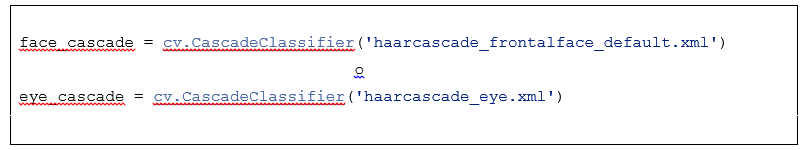
\includegraphics[width=0.99\linewidth]{figures/classifiercode.png}
		\label{fig.classifiercode}
		\end{center}
\end{figure}
Para obtener un objeto Python con el clasificador deseado.

\subsubsection{Eliminación de falsos positivos}
Usar clasificadores en cascada es la mejor manera de reducir la tasa de falsos positivos en la detección. Sin embargo, bajo condiciones cambiantes de luminosidad o entornos con mucho contenido se tienen resultados etiquetados como positivos en casos que claramente no lo son (\textbf{Figura 4.11}):

\begin{figure}[H]
  \begin{center}
    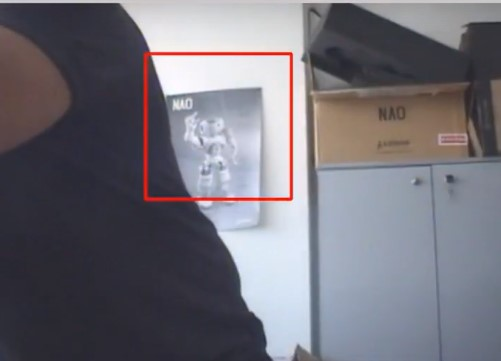
\includegraphics[width=0.70\linewidth]{figures/falsopositivo.jpg}
		\caption{Falso positivo}
		\label{fig.falsopositivo}
		\end{center}
\end{figure}

Proporcionar al sistema un entrenamiento más meticuloso sería la opción ideal para reducir aún más la tasa de error. Sin embargo, las prácticas en este entorno buscan que el alumno se enfrente únicamente a la lógica de control y obtención de datos de los robots, de manera que este problema debe abordarse con código de filtrado de los resultados.

Con ello, tras obtener la posición de todas las caras de la imagen con el método \textit{detectMultiScale} del objeto clasificador de OpenCV (en nuestro caso, \textit{face\_cascade}), aplicamos un filtrado del output que elimine positivos de tamaño inferior a un umbral mínimo, o superior a un umbral máximo para mejorar los resultados. Además, incluimos un clasificador para la detección de ojos que resultará más restrictivo a la hora de hacer una detección final. Finalmente, se utiliza la función \textit{rectangle} del paquete con las coordenadas de la cara para hacer visual la detección. Una vez aplicado el filtro, el resultado cambia (\textbf{Figura 4.12}):

\begin{figure}[H]
  \begin{center}
    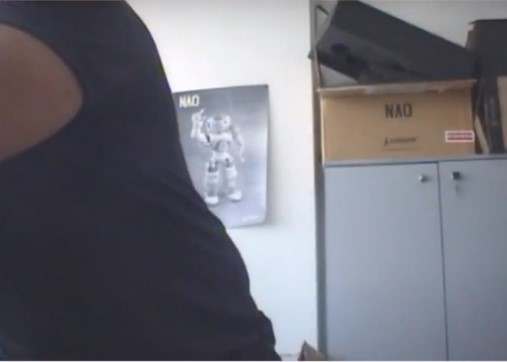
\includegraphics[width=0.70\linewidth]{figures/falsopositivosolved.jpg}
		\caption{Falso positivo solucionado}
		\label{fig.falsopositivosolved}
		\end{center}
\end{figure}

\subsection{Control PT de la cámara}
Dentro del grupo de las cámaras móviles, uno de los grandes subgrupos es el de las cámaras PTZ. Estas siglas indican el control que se puede ejercer sobre la máquina, siendo que se puede modificar el valor que toma en \textit{Pan} (P), el que toma en \textit{Tilt} (T) y el que toma de \textit{zoom} (Z). Nuestra cámara no dispone de \textit{zoom}, se podría decir que consta de un control PT.

Ahora bien, tratándose de control en tiempo real, ¿puede tomar cada componente cualquier valor dentro de los límites del hardware? Evidentemente no. En estos casos debemos contar con el tiempo físico que tarda la cámara en ejecutar el movimiento solicitado. También debe tenerse en cuenta el \textit{buffer} asociado, que encola mensajes hasta que puedan ser atendidos. Si se envía la misma orden dos veces antes de que el hardware sea capaz de terminar la primera (algo muy común), el resultado se traducirá en un “temblor” u oscilación de la cámara entorno a esos valores.

Es por eso que a lo largo del apartado hemos hablado de control gradual. En aplicaciones de este tipo, se hace necesario que el movimiento del cuello mecánico sea a la vez fluido y suave, sin ejecutar movimientos demasiado bruscos, y sin oscilaciones que repercutan en la calidad de la imagen captada, para que el algoritmo pueda seguir funcionando de manera óptima durante los movimientos.
Por ello, hemos decidido implementar un control que trabaje en incrementos o sustracciones pequeñas en grados de los valores \textit{Pan} y \textit{Tilt}. Con ello conseguimos también aprovechar la máxima velocidad de movimiento que ofrece el hardware, sin balanceos, obteniendo un movimiento adecuado en combinación con el tiempo de refresco del hilo de ejecución de algoritmo. En cada iteración, habrá que calcular el centro de la cara detectada y trabajar para que dicho centro coincida con el centro de la imagen captada. En caso de no ser así, se obtendrá el error de posición y se modificarán los valores de control de la cámara de la forma conveniente. En caso de coincidencia, se detendrán los motores y se hará que la cámara permanezca en espera al próximo movimiento.

\subsection{Gestión de la ``No Detección''}
Llegados a este punto se ha llevado a cabo la tarea principal que planteaba esta práctica. Sin embargo, la funcionalidad no es del todo completa. Hemos programado el comportamiento en caso de detección, la eliminación de falsos positivos, la lógica de control y la segmentación pero, ¿qué hace el programa propuesto en caso de no detectar caras en la imagen?

Existen varios caminos posibles:

\begin{itemize}
	\item[--] El primero sería simplemente no hacer nada. El hardware permanece en espera a que una persona entre en escena. Se establece un módulo condicional en el código que detiene los motores en la posición actual si no detecta rostros. No obstante, se puede evolucionar la solución a través de otras vías.
	\item[--] Una segunda opción sería volver a la posición de reposo, de la cual parte la cámara en el primer instante de ejecución. Esto se reflejaría en tener un mayor rango de movimiento cuando una persona vuelva a aparecer en la imagen. Si el clasificador deja de detectar caras cerca del límite físico del cuello mecánico, esta solución lo haría volver al centro, aumentando el margen de movimiento para la próxima detección.
	\item[--] Por último, la solución por la que nos hemos decantado ha sido por iniciar un proceso de búsqueda de rostros dentro del “campo de visión” de la cámara. 
\end{itemize}

Cuando en la imagen no se encuentran secciones que casen con una cara, la cámara esperará 5 segundos como margen para seguir comprobando en las siguientes iteraciones si realmente no hay caras visibles, o si por el contrario se trataba de un error de clasificación. Pasados estos 5 segundos, la cámara comienza un movimiento horizontal (a lo largo del eje X) hacia la derecha, dado que este eje es en el que más probabilidad existe de encontrar una cara, no sólo por las características de las personas (no podemos desplazarnos en vertical, volar), sino también porque es el eje con mayor recorrido del hardware: 328º frente a 60º. Mientras se desplaza sigue ejecutando el algoritmo de detección, de manera que en caso de obtener un positivo, se continúa con la ejecución normal de seguimiento y, en caso contrario, se efectúa el movimiento hasta que se llegue al extremo. Una vez en el extremo, efectúa el mismo movimiento hacia el otro lado. La cámara permanecerá en movimiento en todo momento hasta la detección de una nueva cara.

\section{Experimentación}
En este apartado demostraremos la funcionalidad descrita en los apartados anteriores a través de experimentos realizados para poner a prueba tanto la infraestructura de la práctica, como el nodo y la solución.

\subsection{Ejecución típica}
Se ha preparado un documento de texto (\textit{README.md}) que sirve de guía para que alumno no encuentre dificultades durante la ejecución y el testeo, que incluye también información del API de utilización. 

La forma de ejecutar la práctica es la siguiente:

\begin{enumerate}
	\item Empleamos un primer terminal para inicial el driver de ROS \textit{usb\_cam} (previamente habrá que asegurarse de haber instalado el paquete \textit{ros-kinetic-usb-cam packet}):
	\begin{figure}[H]
		\begin{center}
			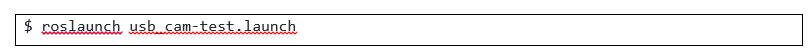
\includegraphics[width=0.95\linewidth]{figures/ffcomando1.png}
			\label{fig.ffcomando1}
		\end{center}
	\end{figure}
	\item Utilizamos un segundo terminal para iniciar el driver \textit{evicam\_driver}:
	\begin{figure}[H]
		\begin{center}
			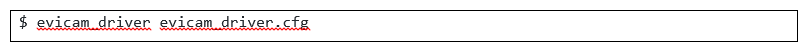
\includegraphics[width=0.95\linewidth]{figures/ffcomando2.png}
			\label{fig.ffcomando2}
		\end{center}
	\end{figure}
	\item 3.	Por último, se lanza en otro terminal el componente \textit{follow\_face}:
	\begin{figure}[H]
		\begin{center}
			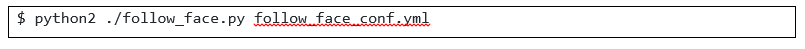
\includegraphics[width=0.95\linewidth]{figures/ffcomando3.png}
			\label{fig.ffcomando3}
		\end{center}
	\end{figure}
\end{enumerate}

Una vez implementada la solución, el \textit{output} debe ser similar al siguiente (\textbf{Figura 4.13}):

\begin{figure}[H]
  \begin{center}
    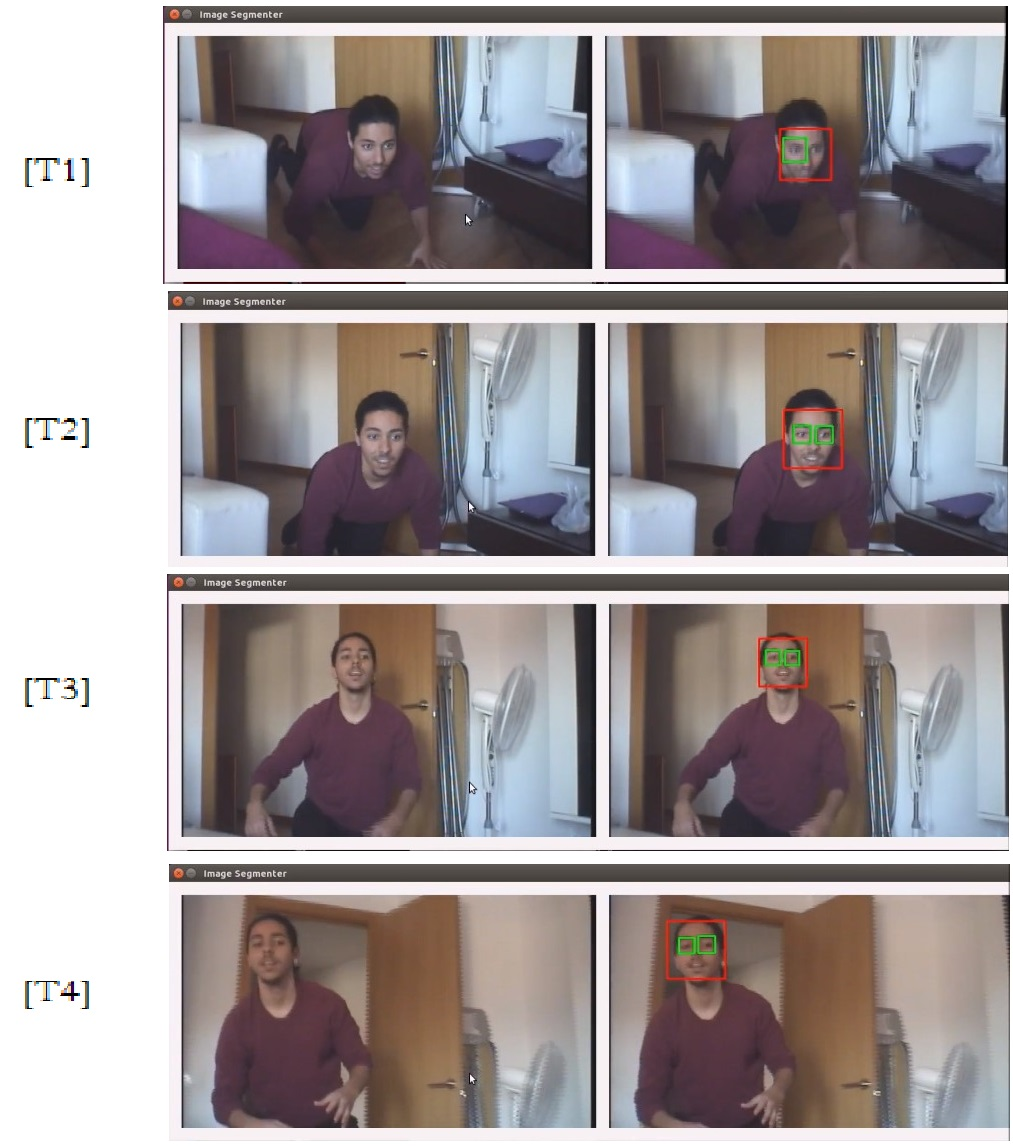
\includegraphics[width=0.98\linewidth]{figures/ffoutput.jpg}
		\caption{Output Follow Face}
		\label{fig.ffoutput}
		\end{center}
\end{figure}

Ejemplos de la ejecución pueden encontrarse en:
 
\url{https://www.youtube.com/watch?v=pdSPnftumf8}, y
 
\url{https://www.youtube.com/watch?v=YZEMIXkXwM0}

\subsection{Comportamiento ante casos extremos}
Como hemos comentado, hemos tratado de poner el algoritmo a prueba para comprobar su validez:

Una primera situación que debimos probar fue la ejecución con movimiento rápido. La persona al frente de la cámara se movió de manera brusca, cambiando de dirección y con subidas y bajadas periódicas. Gracias al movimiento gradual implementado, el algoritmo es capaz de seguir en todo momento el movimiento, salvo en aquellos casos en los que el sujeto se sale bruscamente del plano. 

Por otro lado, probamos la ejecución en situaciones de contraluz. En este caso, el comportamiento empeoraba, ya que la imagen captada, al convertirse a escala de grises, no mostraba apenas diferencia de niveles en pixeles que conforman secciones de la cara que normalmente si presentan dicha diferencia. Esto se debe a las bases de la detección con clasificadores en cascada. Se podría tratar de solucionar incorporando técnicas de detección de color de piel, entre otras.

Por último, en situaciones con muchos candidatos a caras (posters, muñecos y elementos con formas abstractas), el algoritmo se equivocaba el 5\% de las veces, siendo que en el resto de casos escogía el candidato correcto para seguir.

\section{Follow\_Face a través de Jupyter}
En el apartado \textbf{3.6} se introdujo la herramienta Jupyter Notebook,  que permite al usuario crear y compartir documentos que contengan multitud de elementos y widgets programables a través de distintos lenguajes. Hemos aprovechado la funcionalidad de la aplicación para dar un paso más hacia una práctica multiplataforma.
Durante la investigación sobre este proyecto, comprendimos la potencia y prestaciones que ofrece Jupyter, de manera que decidimos adaptar un nodo y una solución a través de esta herramienta. Con él, y utilizando herramientas en desarrollo de JdeRobot y GzWeb\footnote{\url{http://gazebosim.org/gzweb.html}}, más adelante se adaptará un servidor que contenga todo lo necesario para lanzar las prácticas, y que se apoye en interfaces locales como la simulación para alcanzar la independencia de plataforma.

Antes de comenzar, debe instalarse el código del proyecto, proceso del que se detallen las instrucciones en la página oficial del proyecto\footnote{\url{http://jupyter.org/install}}.

Hemos preparado un \textit{Notebook} de Jupyter al que hemos llamado \textit{follow\_face.ipynb}, que junto con algunos cambios en la estructura del nodo académico proporcionan el soporte necesario para tener la misma práctica disponible a través de esta aplicación. En concreto, el nodo programado en el fichero \textit{follow\_face.py} de la práctica original ha sido recodificado para tener estructura de clase Python: la clase \textit{FollowFace}, para poder ser instanciada desde el código del cuadernillo, que detallaremos un poco más adelante. Los cambios más significativos se producen al habernos desecho de la interfaz gráfica, dado que será ahora la propia aplicación la que actúe de interfaz de usuario. Eliminados los componentes gráficos y los widgets que mostraban las imágenes en él, se ha hecho crear una nueva clase (la clase \textit{Printer}, \textbf{Figura 4.14}) que nos permita visualizar las imágenes que el alumno establece a través de métodos disponibles en la clase nodo (\textit{FollowFace}) en la interfaz de Jupyter. Para ello, utilizamos los métodos disponibles en la librería \textit{matplotlib} y su módulo \textit{pyplot},  una colección de funciones cuyo estilo es como un comando que hacen que \textit{matplotlib} funcione como MATLAB en cuanto a representaciones, lo cual simplifica mucho la visualización en la herramienta. 

\begin{figure}[H]
  \begin{center}
    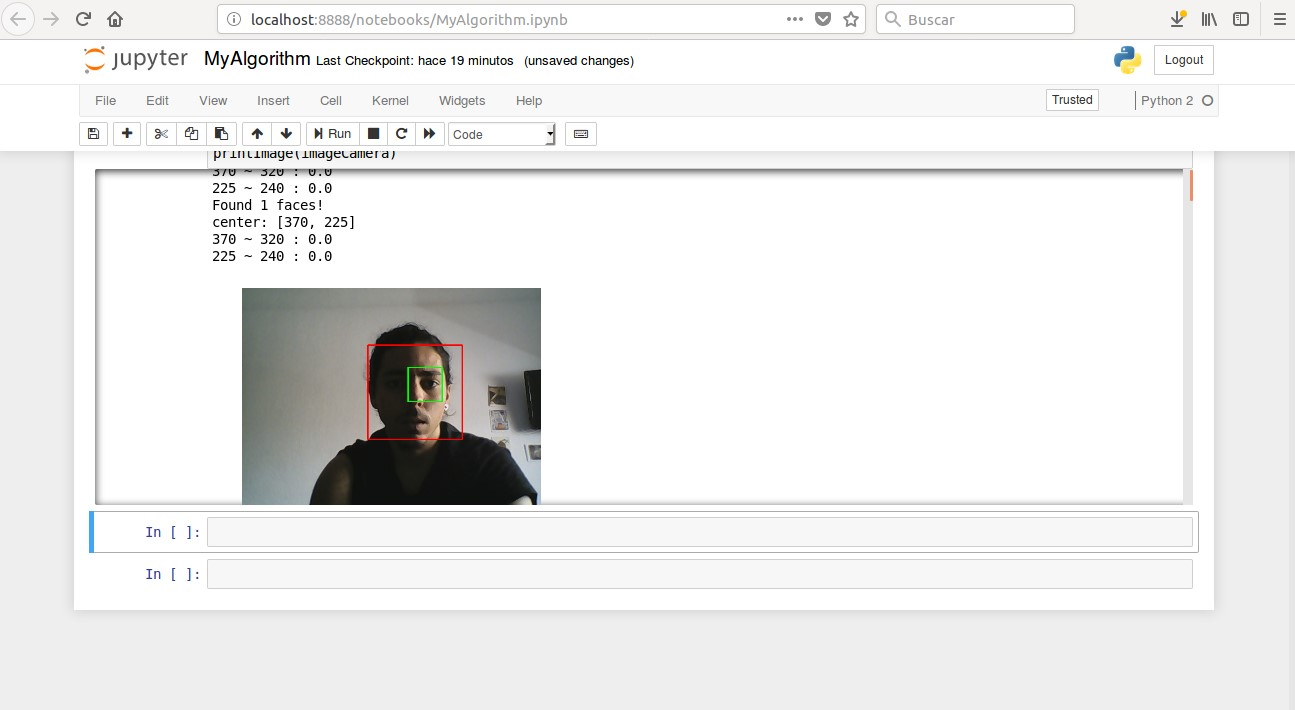
\includegraphics[width=0.98\linewidth]{figures/printer.jpg}
		\caption{Printer}
		\label{fig.printer}
		\end{center}
\end{figure}

Con todo ello, únicamente queda asociar el código del cuadernillo con el del nodo, lo cual conseguimos a través de la librería \textit{types} de Python. Esta librería proporciona acceso a los nombres de algunos tipos de objetos que son utilizados por el intérprete estándar de Python, de manera que podemos modificar el comportamiento normal de los mismos. Utilizaremos la función \textit{MethodType} para hacer corresponder la función que el estudiante retoca desde la aplicación de Jupyter con el método que realiza el cómputo en el hilo de algoritmo del nodo académico modificado. Por último, hemos de recordar que necesitamos de la intervención de dos \textit{drivers} para controlar la cámara de la que disponemos, de manera que la adaptación del nodo incorpora el lanzamiento de dos subprocesos, uno para cada \textit{driver}, a través de la librería \textit{subprocess}, que permite generar nuevos procesos y conectarse a sus tuberías de entrada / salida / error, además de obtener sus códigos de retorno. Con esto, y unas pequeñas incorporaciones al nodo para poder parar o ejecutar el algoritmo desde Jupyter, completamos la práctica a través de la aplicación. 

Entrando ya en el cuadernillo o \textit{Notebook} generado (\textbf{Figura 4.15}), éste no sólo incorpora celdillas de código ejecutable embebidas, sino que también incluye imágenes representativas y texto descriptivo para orientar al alumno en todo momento (durante la ejecución, aportando información adicional para abordar la práctica y explicando el API de utilización con los nuevos métodos de visualización y actualización del código. 

Así, el alumno puede abordar la práctica de manera totalmente guiada, y ejecutar los distintos pasos que va abordando para observar su salida, con herramientas disponibles para depurar errores o matizar su solución.

\begin{figure}[H]
  \begin{center}
    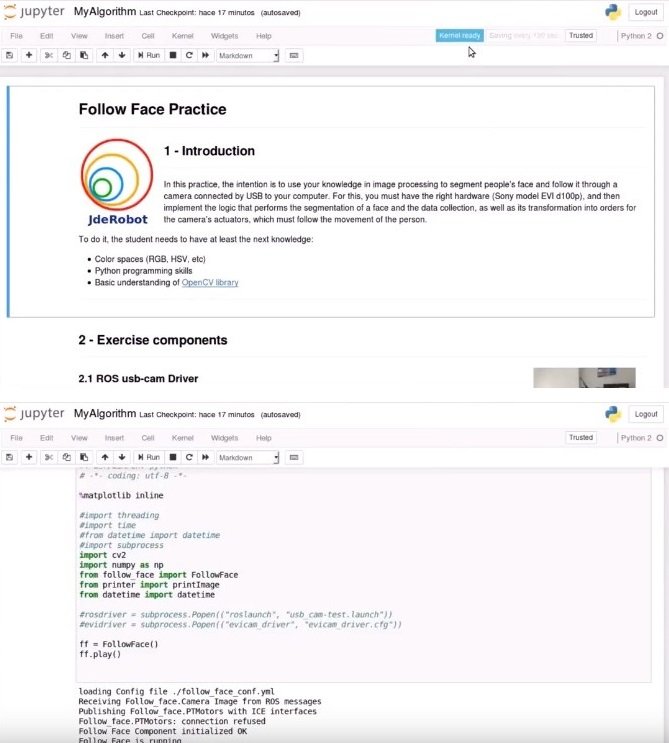
\includegraphics[width=0.98\linewidth]{figures/notebookff.jpg}
		\caption{Notebook Follow Face}
		\label{fig.notebook}
		\end{center}
\end{figure}

Un vídeo demostrando el comportamiento de la práctica a través de Jupyter se puede ver en:

\url{https://www.youtube.com/watch?v=9fOqkw7fUHg}

